\documentclass[12pt]{article}

\usepackage[margin=1in]{geometry}
\usepackage{amsmath, amssymb}
\usepackage{amsfonts}
\usepackage{braket, units, enumitem}
\usepackage{todonotes}
\usepackage{graphicx}
\usepackage{mdframed}
\usepackage{tikz}
\usepackage{tikz-cd}
\usetikzlibrary{decorations.pathmorphing}
\usetikzlibrary{matrix}


\newmdenv[
  topline=false,
  bottomline=false,
  rightline=false,
  skipabove=\topsep,
  skipbelow=\topsep
]{leftrule}

\usepackage{tikz}
\newcommand*\circled[1]{\tikz[baseline=(char.base)]{
            \node[shape=circle,draw,inner sep=2pt] (char) {#1};}}
\let\oldBC\because
\renewcommand\because{\raisebox{0.75pt}{$\quad\oldBC\quad$}}

\newcommand{\fig}[3]{
    \begin{center}
    \includegraphics[scale=#3]{#1} \\
    #2 \\
    \end{center}
}

\begin{document}

\newcounter{set}
\setcounter{set}{1}
\newcounter{problem}[set]
\newcommand{\problem}{{\vspace{2\baselineskip}\noindent\large \bfseries Problem~\arabic{set}:}\\\refstepcounter{set}}
\newcommand{\problemsub}{\refstepcounter{problem}{\vspace{2\baselineskip}\noindent\large \bfseries Problem~\arabic{set} \roman{problem}:}\\}
\newcommand{\problemasub}{\refstepcounter{problem}{\vspace{2\baselineskip}\noindent\large \bfseries Problem~\arabic{set}\alph{problem}:}\\}

\title{CS 486 - A5}

\author{Alexander Maguire \\
amaguire@uwaterloo.ca \\
20396195}

\setlength{\parindent}{0pt}
\twocolumn
\maketitle

\problemasub

The code to generate this section is included as \texttt{policy.hs}. \\

\begin{tabular}{cccc}
    206 $\leftarrow$ & 147 $\leftarrow$ & 105 $\leftarrow$ \\
    147 $\uparrow$ & 105 $\uparrow$ & 74 $\uparrow$ \\
    116 $\uparrow$ & 82 $\uparrow$ & 58 $\uparrow$
\end{tabular}

\problemasub
\begin{tabular}{ccc}
    6 $\rightarrow$ & 4 $\rightarrow$ & 2 $\downarrow$ \\
    12 $\rightarrow$ & 8 $\uparrow$ & 4 $\uparrow$ \\
    19 $\uparrow$ & 12 $\uparrow$ & 8 $\uparrow$
\end{tabular}

\problemasub
\begin{tabular}{ccc}
    9 $\rightarrow$ & 5 $\rightarrow$ & 3 $\downarrow$ \\
    12 $\uparrow$ & 8 $\uparrow$ & 4 $\uparrow$ \\
    19 $\uparrow$ & 12 $\uparrow$ & 8 $\uparrow$
\end{tabular}

\problemasub
\begin{tabular}{ccc}
    12 $\rightarrow$ & 7 $\rightarrow$ & 4 $\downarrow$ \\
    12 $\uparrow$ & 8 $\uparrow$ & 4 $\uparrow$ \\
    19 $\uparrow$ & 12 $\uparrow$ & 8 $\uparrow$
\end{tabular}



\newpage
\stepcounter{set}
\problem

\begin{tabular}{cccc}
    {}   & N      & C      & J      \\
    N    & 73, 25 & 57, 42 & 66, 32 \\
    C    & 80, 26 & 35, 12 & 32, 54 \\
    J    & 28, 27 & 63, 31 & 54, 29 \\
\end{tabular} \vspace{5mm} \\

\begin{tabular}{cccc}
    {}   & C      & J      \\
    N    & 57, 42 & 66, 32 \\
    C    & 35, 12 & 32, 54 \\
    J    & 63, 31 & 54, 29 \\
\end{tabular} \vspace{5mm}

\begin{tabular}{cccc}
    {}   & C      & J      \\
    N    & 57, 42 & 66, 32 \\
    J    & 63, 31 & 54, 29 \\
\end{tabular} \vspace{5mm}

\begin{tabular}{cccc}
    {}   & C      \\
    N    & 57, 42 \\
    J    & 63, 31 \\
\end{tabular} \vspace{5mm}

\begin{tabular}{cccc}
    {}   & C      \\
    J    & 63, 31 \\
\end{tabular} \vspace{5mm} \\

This is a Nash equilibrium, because given $(J,C)$, player 1 can't do better by changing from $J$, and player 2 can't do
better by changing from $C$.

\newpage
\problem

Leave-one-out cross-validation is the process of partitioning your dataset of $n$ elements into a training set with
$n-1$ elements and a testing set of with 1 element. The number of positive examples is the same as the number
of negative examples in the original dataset.

Without loss of generality, assume the sample taken for the testing dataset is classified positive, so its majority is
positive. The training set now contains $n/2 - 1$ positive examples, and $n/2$ negative examples, so its majority is
negative. Leave-one-out cross-validation will now always score zero by the construction of the training set.

\problemsub
The code for this section is attached as \\ \texttt{tree.hs}.

\problemsub
\begin{figure}[h!]
  \caption{The decision tree for horses}
  \centering
    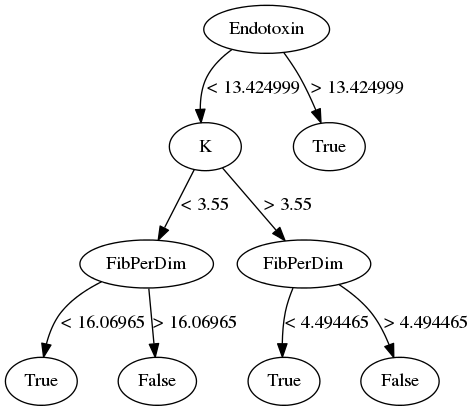
\includegraphics[width=0.5\textwidth]{horse-graph.png}
\end{figure}

\newpage
\problemsub
The algorithm classifies 132 examples of the training set correctly.

\problemsub
The algorithm classifies 13 examples of the training set correctly.

\problemsub
I use the information gain by trying every possible threshold value over all attributes, and selecting the one which
provides the highest information gain.

\stepcounter{set}
\problemsub
The code for this section is identical to question 4.

\problemsub
The generated decision tree is included in the appendix as Figure 2.
\begin{figure*}
  \caption{The decision tree for math}
  \centering
  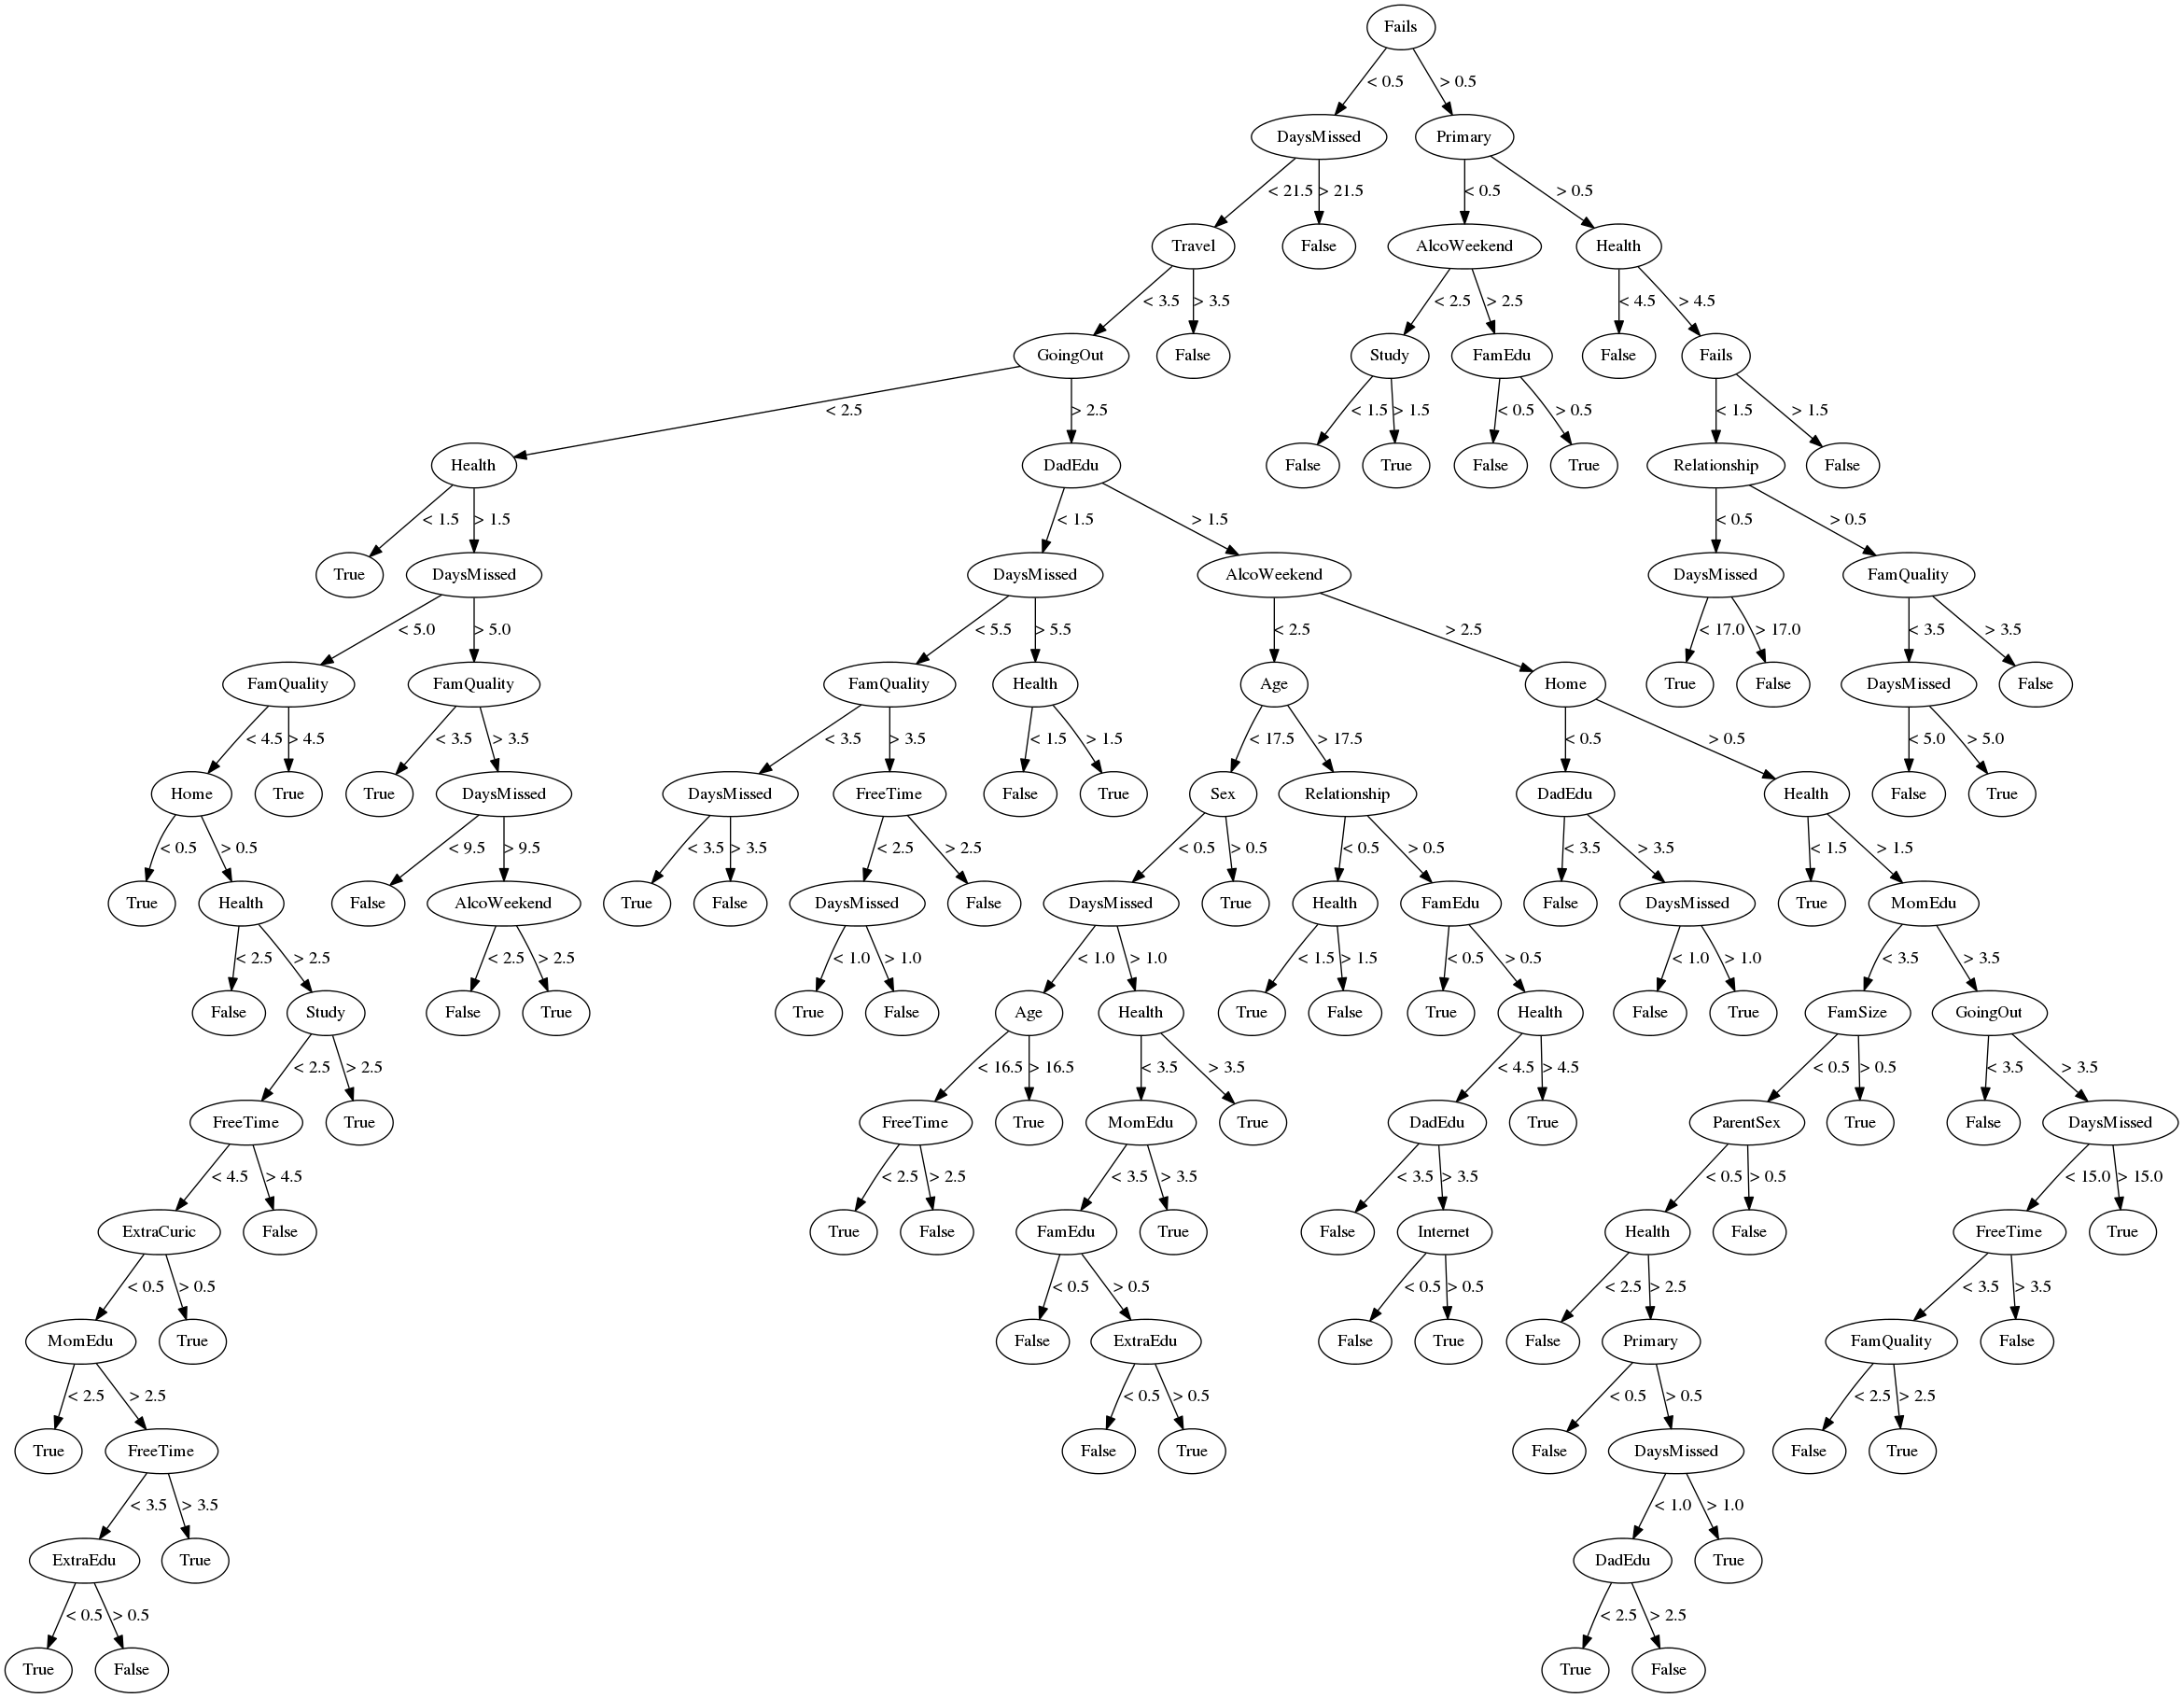
\includegraphics[width=\textwidth]{math-graph.png}
\end{figure*}

\problemsub
The algorithm classifies 249 examples of the training set correctly.

\problemsub
The algorithm classifies 84 examples of the testing set correctly.

\problemsub
There is a significant difference in the classification results between the training and testing sets. Presumably this
is because the none of the provided features accurately track the classification, but instead are only sort of related.

\end{document}
